\documentclass{standalone}

\usepackage{tikz}
\usetikzlibrary{arrows}
\usetikzlibrary{decorations.markings}
\usetikzlibrary{calc}
\usetikzlibrary{shapes.geometric}
\usepackage{standalone}

\begin{document}

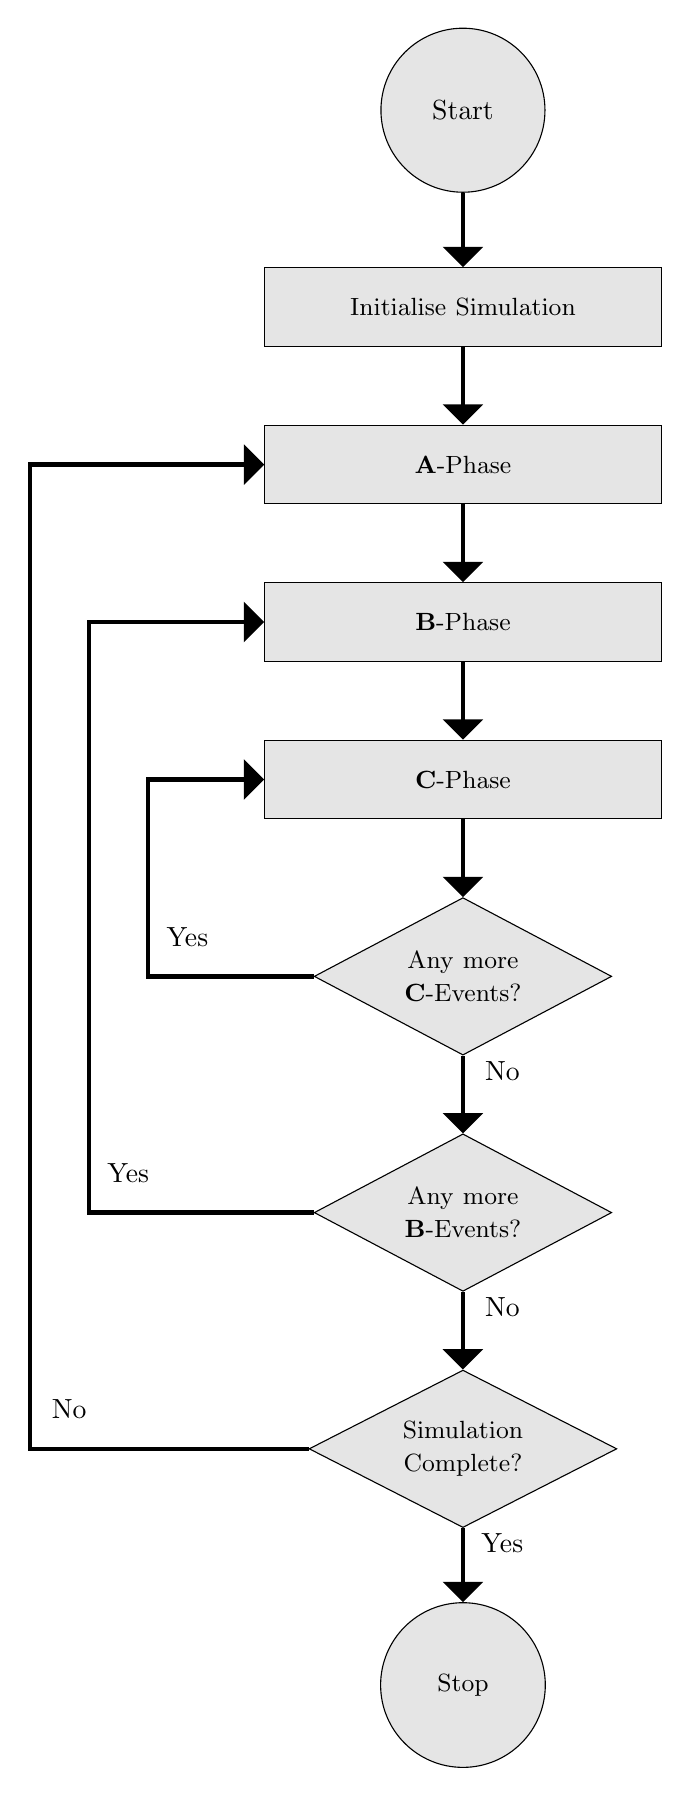
\begin{tikzpicture}

\node[align=center] (start) [style={minimum size=2cm, text width=1.8cm, draw=black,fill=black!10,text=black,shape=circle}] at (0, 19) {Start};
\node[align=center] (initial) [style={minimum width=5cm, minimum height=1cm, text width=4.8cm, draw=black,fill=black!10,text=black,shape=rectangle}] at (0, 16.5) {\small{Initialise Simulation}};
\node[align=center] (Aphase) [style={minimum width=5cm, minimum height=1cm, text width=4.8cm, draw=black,fill=black!10,text=black,shape=rectangle}] at (0, 14.5) {\small{\textbf{A}-Phase}};
\node[align=center] (Bphase) [style={minimum width=5cm, minimum height=1cm, text width=4.8cm, draw=black,fill=black!10,text=black,shape=rectangle}] at (0, 12.5) {\small{\textbf{B}-Phase}};
\node[align=center] (Cphase) [style={minimum width=5cm, minimum height=1cm, text width=4.8cm, draw=black,fill=black!10,text=black,shape=rectangle}] at (0, 10.5) {\small{\textbf{C}-Phase}};
\node[align=center] (anymoreC) [style={minimum size=2cm, text width=1.8cm, draw=black,fill=black!10,text=black,shape=diamond, aspect=2}] at (0, 8) {\small{Any more \textbf{C}-Events?}};
\node[align=center] (anymoreB) [style={minimum size=2cm, text width=1.8cm, draw=black,fill=black!10,text=black,shape=diamond, aspect=2}] at (0, 5) {\small{Any more \textbf{B}-Events?}};
\node[align=center] (isend) [style={minimum size=2cm, text width=1.8cm, draw=black,fill=black!10,text=black,shape=diamond, aspect=2}] at (0, 2) {\small{Simulation Complete?}};
\node[align=center] (stop) [style={minimum size=2cm, text width=1.8cm, draw=black,fill=black!10,text=black,shape=circle}] at (0, -1) {\small{Stop}};

\draw[ultra thick, -triangle 90] (start) -- (initial);
\draw[ultra thick, -triangle 90] (initial) -- (Aphase);
\draw[ultra thick, -triangle 90] (Aphase) -- (Bphase);
\draw[ultra thick, -triangle 90] (Bphase) -- (Cphase);
\draw[ultra thick, -triangle 90] (Cphase) -- (anymoreC);
\draw[ultra thick, -triangle 90] (anymoreC) -- (anymoreB);
\draw[ultra thick, -triangle 90] (anymoreB) -- (isend);
\draw[ultra thick, -triangle 90] (isend) -- (stop);

\draw[ultra thick, -triangle 90] (anymoreC) -- (-4, 8) -- (-4, 10.5) -- (Cphase);
\draw[ultra thick, -triangle 90] (anymoreB) -- (-4.75, 5) -- (-4.75, 12.5) -- (Bphase);
\draw[ultra thick, -triangle 90] (isend) -- (-5.5, 2) -- (-5.5, 14.5) -- (Aphase);

\node at (0.5, 6.8) {No};
\node at (-5, 2.5) {No};
\node at (0.5, 3.8) {No};
\node at (-3.5, 8.5) {Yes};
\node at (-4.25, 5.5) {Yes};
\node at (0.5, 0.8) {Yes};



\end{tikzpicture}

\end{document}
